\chapter{Diseño e Implementación} % Main chapter title

\label{Chapter3} % Change X to a consecutive number; for referencing this chapter elsewhere, use \ref{ChapterX}
\definecolor{mygreen}{rgb}{0,0.6,0}
\definecolor{mygray}{rgb}{0.5,0.5,0.5}
\definecolor{mymauve}{rgb}{0.58,0,0.82}

\lstset{ %
  backgroundcolor=\color{white},   % choose the background color; you must add \usepackage{color} or \usepackage{xcolor}
  basicstyle=\footnotesize,        % the size of the fonts that are used for the code
  breakatwhitespace=false,         % sets if automatic breaks should only happen at whitespace
  breaklines=true,                 % sets automatic line breaking
  captionpos=b,                    % sets the caption-position to bottom
  commentstyle=\color{mygreen},    % comment style
  deletekeywords={...},            % if you want to delete keywords from the given language
  %escapeinside={\%*}{*)},          % if you want to add LaTeX within your code
  %extendedchars=true,              % lets you use non-ASCII characters; for 8-bits encodings only, does not work with UTF-8
  %frame=single,	                   % adds a frame around the code
  keepspaces=true,                 % keeps spaces in text, useful for keeping indentation of code (possibly needs columns=flexible)
  keywordstyle=\color{blue},       % keyword style
  language=Java,					% the language of the code
  %otherkeywords={*,...},           % if you want to add more keywords to the set
  numbers=left,                    % where to put the line-numbers; possible values are (none, left, right)
  numbersep=5pt,                   % how far the line-numbers are from the code
  numberstyle=\tiny\color{mygray}, % the style that is used for the line-numbers
  rulecolor=\color{black},         % if not set, the frame-color may be changed on line-breaks within not-black text (e.g. comments (green here))
  showspaces=false,                % show spaces everywhere adding particular underscores; it overrides 'showstringspaces'
  showstringspaces=false,          % underline spaces within strings only
  showtabs=false,                  % show tabs within strings adding particular underscores
  stepnumber=1,                    % the step between two line-numbers. If it's 1, each line will be numbered
  stringstyle=\color{mymauve},     % string literal style
  tabsize=2,	                   % sets default tabsize to 2 spaces
  title=\lstname,                   % show the filename of files included with \lstinputlisting; also try caption instead of title
  morecomment=[s]{/*}{*/}%
}

En este capítulo se describe la implementación y la estructura de software adoptada para el diseño de CIAABOT.
%----------------------------------------------------------------------------------------
%	SECTION 1
%----------------------------------------------------------------------------------------
\section{Estructura del software}
%----------------------------------------------------------------------------------------
En esta sección se detallan y justifican las decisiones de diseño tomadas. También se desarrollará en profundidad el diseño del software del IDE.

\subsection{Estructura de un proyecto base}
\label{subsec:estructura-proyecto}
Cuando se crea un proyecto nuevo en CIAABOT IDE, se crea una carpeta con varias subcarpetas y archivos. En la figura \ref{fig:estructura-archivos} se observa esta estructura simplificada. Está basada en la estructura de archivos que se utiliza en el Firmware V2 de la CIAA.

Firmware V2 es un proyecto, basado en makefile para el desarrollo de software en C, especialmente enfocado en sistemas embebidos, particularmente microcontroladores. Actualmente provee soporte para:

\begin{itemize}
\item LPC11U68 (Cortex M0+).
\item LPC1769 (Cortex M3).
\item LPC4337 (Cortex M4 y M0).
\item LPC54102 (Cortex M4 y M0+).
\end{itemize}

El Firmware V2 e basa principalmente en el workspace del Esp. Ing. Pablo Ridolfi y la sAPI del Ing. Eric Pernía, que es el director del presente trabajo final.

En la estructura del proyecto se encuentra el archivo con extensión \texttt{.cbp}. Éste contiene la información del proyecto, su nombre, el modelo de CIAABOT utilizado y el diagrama en bloques. Los archivos \texttt{config.mk} y \texttt{Makefile} se utilizan para la compilación del código C y la descarga del mismo a la placa.

En el directorio \texttt{libs} se encuentran las diferentes bibliotecas que incluye el proyecto. En \texttt{lpc\_chip\_43xx} están las bibliotecas de LPCOpen para el microcontrolador LPC4337, provistas por el fabricante. En \texttt{lpc\_board\_ciaa\_edu\_4337} está la biblioteca a nivel de placa puntualmente para manejar la placa EDU-CIAA-NXP.

En la carpeta \texttt{sapi} se encuentra la biblioteca sAPI. Esta biblioteca permite manejar varios periféricos del microcontrolador de manera simplificada. Estos son:

\begin{itemize}
\item Interrupciones.
\item SysTick.
\item GPIO.
\item UART.
\item ADC.
\item DAC.
\item $I^2C$.
\item SPI.
\item RTC.
\item SCT.
\item Timers.
\end{itemize}

Además incluye funciones avanzadas de conversión de datos, impresión formateada por UART, manejo de displays 7 segmentos, teclados matriciales, servos y PWM entre otras.

Finalmente, la carpeta \texttt{app} contiene la aplicación de usuario. Puntualmente el archivo \texttt{main.c} es el que se actualiza al realizar modificaciones en el editor de bloques del IDE.

\begin{minipage}{\linewidth}
\begin{verbatim}

        Estructura de un proyecto de CIAABOT IDE
        |   config.mk
        |   Makefile
        |   mi-proyecto.cbp
        |
        |---app
        |   |---inc
        |   |       programa.h
        |   |
        |   |---src
        |           main.c
        |
        |---libs
        |   |---lpc_board_ciaa_edu_4337
        |   |   |---inc
        |   |   |---src
        |   |
        |   |---lpc_chip_43xx
        |   |   |---inc
        |   |   |---src
        |   |---sapi
        |       |---inc
        |       |---src
        |
        |---scripts
\end{verbatim}
\label{fig:estructura-archivos}
\captionof{figure}{Estructura simplificada de un proyecto base.}
\end{minipage}



\subsection{Editor de código en bloques}
El editor de bloques es la sección central de CIAABOT IDE. Aquí el usuario toma e interconecta los diferentes bloques que permiten realizar los programas. Se utilizó la biblioteca de JavaScript Blockly de Google \citep{blockly}, realizada por Neil Fraser entre otros.

Blockly es una biblioteca que utiliza bloques gráficos encastrables para representar los conceptos de código como variables, espresiones lógicas, bucles y más. Permite que los usuarios apliquen conocimientos de programación sin preocuparse por una sintaxis específica.

Durante el proceso de selección de la biblioteca para armar el editor gráfico, se seleccionó Blockly por las siguientes ventajas que presenta:

\begin{itemize}
\item Permite exportar el código simplemente.
\item Es un proyecto de software libre.
\item Es ampliable, ya que se pueden agregar bloques personalizados.
\item Ha sido traducido a más de 40 idiomas, y permite una traducción de los bloques propios.
\end{itemize}

Esta biblioteca permite, por un lado, definir bloques con diferentes tipos de conexiones y parámetros, y por otro armar generadores que reciban los bloques y generen código. Nativamente Blockly soporta varios lenguajes, pero no C. Para eso, se utilizó parte del desarrollo de Fred Lin, BlocklyDuino \citep{blocklyduino}, que resolvió varios de las estructuras típicas de C.

Blockly permite definir los bloques independientemente de los generadores de código. La definición implica la forma que tendrá el bloque para el usuario (colores, secciones, textos, tipos de bloques admitidos en cada sección y configuraciones especiales).

Para definir los bloques se utilizan archivos JavaScript y una sintaxis especial. Por ejemplo, así se define el bloque de retardo bloqueante:


\begin{lstlisting}[caption=Definición del bloque de retardo bloqueante.]

Blockly.Blocks['ciaa_sapi_blocking_delay'] = {
    init: function () {
        this.appendValueInput("delay_time")
            .setCheck("Number")
            .appendField("Esperar ticks");
        this.setPreviousStatement(true, null);
        this.setNextStatement(true, null);
        this.setColour(230);
        this.setTooltip('Retardo bloqueante');
        this.setHelpUrl('');
    }
};
\end{lstlisting}

Es posible definir varios generadores de código para los mismos bloques. Esto significa que un mismo programa podría ser traducido a varios lenguajes según la necesidad. A modo de ejemplo se muestra cómo se puede definir el generador de código para lenguaje C para el bloque de retardo bloqueante:

\begin{lstlisting}[caption=Generador de código en lenguaje C para el retardo bloqueante.]

Blockly.CiaaSapi.ciaa_sapi_blocking_delay = function() {
  var delay_time = Blockly.CiaaSapi.valueToCode(this, 'delay_time', Blockly.CiaaSapi.ORDER_ATOMIC) || '2000';
  var code = 'delay(' + delay_time + ');\n';
  return code;
};
\end{lstlisting}

Si se observa la definición del bloque, se está agregando una entrada del tipo \emph{value} llamada \emph{delay\_time}, que luego en el generador es tomada y utilizada como argumento de la función \emph{delay} de la sAPI.

Internamente en el programa, cuando el usuario modifica el esquema de bloques, se llama a la biblioteca. Esta recibe como parámetro el nuevo diagrama en formato XML (\emph{eXtensible Markup Language}, Lenguaje de Marcado Extensible), y el generador de código que se desea aplicar. Como resultado se obtiene una cadena de caracteres que es el código generado. Este código puede suponerse sintácticamente correcto, y en la mayoría de los casos compilará sin problemas.

Como se aprecia en la figura \ref{fig:secciones-editor}, el editor tiene tres secciones principales: Una barra de acciones, una caja de herramientas y el área de edición.

\begin{figure}[h]
\centering
\includegraphics[scale=.5]{./Figures/editor.jpg}
\caption{Secciones del editor de bloques.}
\label{fig:secciones-editor}
\end{figure}

En la figura \ref{fig:barra-acciones} se presenta una descripción detallada de las acciones disponibles en la Barra de Acciones. La caja de herramientas divide los bloques en categorías:

\begin{itemize}
\item Lógica
\item Entradas / Salidas.
\item Servo.
\item Tiempo.
\item Control.
\item Variables.
\item Funciones.
\item Matemática.
\item Texto
\end{itemize}

\begin{figure}[h]
\centering
\includegraphics[scale=.8]{./Figures/barra-acciones.jpg}
\caption{Detalle de la barra de acciones.}
\label{fig:barra-acciones}
\end{figure}

Los bloques se arrastran al área de edición y se interconectan con los demás. Hay diferentes tipos de bloques, según su tipo de conexión. Hay bloques que admiten solamente conexiones superior e inferior (figura \ref{fig:bloque:esperar}), como el de \emph{Esperar x segundos}. Estos bloques no retornan ningún valor, ni contienen otros bloques internamente. En el caso de este bloque, admite dos configuraciones: Unidad de tiempo en la que se esperará y cantidad de esas unidades. La unidad se selecciona con una lista de valores predeterminados, y la cantidad admite un bloque numérico (puede ser un número inmediato o el resultado de alguna operación).


\begin{figure}[h]
\centering
\includegraphics[scale=1]{./Figures/bloque-esperar.jpg}
\caption{Bloque Esperar x segundos.}
\label{fig:bloque:esperar}
\end{figure}

Otros bloques, como la lectura del periférico conversor analógico a digital, retornan un valor que es tomado por algún bloque como argumento (por ejemplo una comparación). Este tipo de bloque se muestra en la figura \ref{fig:bloque:adc}. No admite conexiones superior ni inferior.

\begin{figure}[H]
\centering
\includegraphics[scale=1]{./Figures/bloque-adc.jpg}
\caption{Bloque Leer conversor analógico a digital.}
\label{fig:bloque:adc}
\end{figure}

Hay algunos bloques más complejos como el \emph{Si...hacer} que permiten una configuración avanzada de la forma que presentan y los bloques que admiten. En la figura \ref{fig:bloque:si} se observa cómo se configura este bloque para que admita una segunda sección de bloques que se ejecutan de no cumplirse la condición estipulada en \emph{Si...}.

\begin{figure}[H]
\centering
\includegraphics[scale=.8]{./Figures/bloque-si.jpg}
\caption{Bloque Condicional.}
\label{fig:bloque:si}
\end{figure}

A modo de ejemplo, en la figura \ref{fig:codigo-servo-bloques} cómo se armaría en bloques el código para el barrido angular de un servomotor.

\begin{figure}[H]
\centering
\includegraphics[scale=.8]{./Figures/ejemplo-servo.jpg}
\caption{Ejemplo de código en bloques para el barrido de un servo.}
\label{fig:codigo-servo-bloques}
\end{figure}

El código de salida de la figura \ref{fig:codigo-servo-bloques} se muestra a continuación:


\begin{lstlisting}[caption={Salida del código en bloques de la figura \ref{fig:codigo-servo-bloques}.}\label{cod:codigo-servo-c}] 
#include "sapi.h"
CONSOLE_PRINT_ENABLE

inline void setup(void) {
  servoConfig(0, SERVO_ENABLE);
  servoConfig(SERVO0, SERVO_ENABLE_OUTPUT);
}


void main(void) {
	// Inicializa placa
	boardConfig();

	// Habilita cuenta de tick cada 1ms
	tickConfig(1, 0);

	// Inicializaciones del usuario
	setup();

    while (TRUE) {
       servoWrite(SERVO0, 0);
       delay(1000 * 1);
       servoWrite(SERVO0, 180);
       delay(1000 * 1);
    }
}

\end{lstlisting}

\subsection{Definición del lenguaje específico}
Un DSL (\emph{Domain-specific language}, Lenguaje de dominio específico) es un lenguaje de programación o especificación dedicado a resolver un problema en particular, representar un problema específico y proveer una técnica para solucionar esa situación particular. Ejemplos de esto incluyen Verilog (descripción de hardware), R y S para estadísticas, SQL para consultas a bases de datos, entre otros. \citep{DSL}.

A la hora de diseñar los bloques que se incluirían en CIAABOT IDE se puso como foco principal su uso didáctico, que fuera de fácil comprensión y que el esquema de bloques resultante pudiese leerse con una fluidez similar al habla. Para esto se debió hacer una definición del lenguaje CIAABOT.

La versión actual se acotó a una serie de limitaciones, por cuestiones de tiempo. Estas son:
\begin{itemize}
\item Pines con funcionalidades fijas.
\item Periféricos disponibles: GPIO, ADC, DAC, UART, $I^2C$, PWM, Servo.
\item Todas las variables del usuario son globales.
\item Las funciones (bloques de usuario) no retornan valores (son procedimientos).
\item El tipo de dato \emph{string} se utiliza únicamente para crear literales para enviar por UART.
\end{itemize}

En la tabla \ref{tab:definicion-lenguaje} se lista la versión 1.0.0 de la definición del lenguaje CIAABOT. Los bloques se agruparon por categoría.

\begin{longtable}[c]{ll}
\caption{Definición del lenguaje CIAABOT v1.0.0}
\label{tab:definicion-lenguaje}\\
\hline
\multicolumn{2}{c}{\textbf{API}}                                                                                                                                                                                                    \\ \hline
\endhead
%
\multicolumn{1}{l}{\textbf{Nombre/categoría}} & \multicolumn{1}{c}{\textbf{Traducción}}                                                                                                                                             \\ \hline
\textbf{Control de ejecución}                 &                                                                                                                                                                                     \\ \hline
if                                            & Si \textless condicion booleana\textgreater hacer {[}{]}                                                                                                                            \\
else                                          & Si no hacer {[}{]}                                                                                                                                                                  \\
switch, case, default                         & \makecell[ll]{Si \textless var\textgreater es igual a \textless literal\textgreater hacer {[}{]} si es distinto \\ a los anteriores hacer {[}{]}}                                                     \\ \hline
\textbf{Bucles de repetición}                 &                                                                                                                                                                                     \\ \hline
do                                            & Hacer {[}{]} y repetir \textless mientras/hasta\textgreater \textless condicion booleana\textgreater                                                                                \\
while                                         & Repetir {[}{]} \textless mientras/hasta\textgreater \textless condicion booleana\textgreater                                                                                        \\
for                                           & \makecell[ll]{Iterar \textless var int\textgreater desde \textless literal int\textgreater hasta \textless literal int\textgreater \\ incrementando \textless literal int\textgreater y hacer {[}{]} }\\

                                              & Repetir {[}{]} \textless literal int\textgreater veces                                                                                                                              \\
while(TRUE)                                   & Repetir para siempre {[} {]}                                                                                                                                                        \\ \hline
\textbf{Manejo de tiempos}                    &                                                                                                                                                                                     \\ \hline
tickRead                                      & Leer base de tiempo (ms)                                                                                                                                                            \\
tickWrite                                     & Escribir base de tiempo (ms)                                                                                                                                                        \\
delay                                         & Esperar durante \textless int\textgreater \textless unidad\textgreater                                                                                                              \\
delay\_t \textless var\textgreater;           & Crear temporizador con nombre \textless var\textgreater                                                                                                                             \\
delayConfig                                   & Iniciar \textless temporizador\textgreater con \textless int\textgreater \textless unidad\textgreater                                                                               \\
delayRead                                     & Leer \textless temporizador\textgreater                                                                                                                                             \\
delayWrite                                    & Escribir \textless temporizador\textgreater con \textless int\textgreater \textless unidad\textgreater                                                                              \\ \hline
\textbf{GPIO}                                 &                                                                                                                                                                                     \\ \hline
gpioRead                                      & Leer estado del GPIO \textless GPIOi, TECi, LEDi\textgreater                                                                                                                        \\
gpioWrite                                     & \makecell[ll]{Establecer estado del GPIO \textless GPIOi , LEDi\textgreater \\ en \textless encender/apagar\textgreater }                                                                              \\
gpioToggle                                    & Invertir el estado del pin \textless GPIOi, LEDi\textgreater                                                                                                                        \\ \hline
\textbf{ADC}                                  &                                                                                                                                                                                     \\ \hline
adcRead                                       & Leer ADC \textless ADCi\textgreater                                                                                                                                                 \\ \hline
\textbf{DAC}                                  &                                                                                                                                                                                     \\ \hline
dacWtite                                      & Establecer DAC \textless DACi\textgreater al valor \textless literal int\textgreater                                                                                                \\ \hline
\textbf{UART}                                 &                                                                                                                                                                                     \\ \hline
uartReadByte                                  & Recibir byte desde UART \textless UARTi\textgreater                                                                                                                                 \\
uartWriteByte                                 & Enviar byte \textless var/literal\textgreater por UART \textless UARTi\textgreater                                                                                                  \\
uartWriteString                               & Enviar texto \textless Texto\textgreater por UART \textless UARTi\textgreater                                                                                                       \\ \hline
\textbf{PWM}                                  &                                                                                                                                                                                     \\ \hline
pwmWrite                                      & \makecell[ll]{Establecer ciclo de trabajo de PWM \textless PWMi\textgreater en \textless \\ literal int\textgreater \%}                                                                               \\ \hline
\textbf{SERVO}                                &                                                                                                                                                                                     \\ \hline
servoWrite                                    & Establecer ángulo de SERVO \textless SERVOi\textgreater a \textless literal int\textgreater                                                                                         \\
servoRead                                     & Leer ángulo de SERVO \textless SERVOi\textgreater                                                                                                                                  
\end{longtable}

\subsection{Servicios}
Para el desarrollo de CIAABOT IDE se utilizó \emph{Electron}\citep{electron}, una biblioteca de código abierto desarrollada por GitHub para armar aplicaciones de escritorio multiplataforma utilizando tecnologías web como HTML, CSS y JavaScript (o TypeScript). De esta manera, se puede simplificar y reutilizar el diseño de una aplicación, ya que con mínimas consideraciones se puede desarrollar una aplicación de escritorio una vez que compile para varios sistemas operativos. Esto lo logra combinando el navegador Chromium de Google con \emph{NodeJS} \citep{nodejs}. Se puede observar en la figura \ref{fig:ideLayers} las tecnologías utilizadas para el desarrollo de CIAABOT IDE, en un formato de capas, que finaliza con la interacción de la aplicación con el sistema operativo.

\begin{center}
    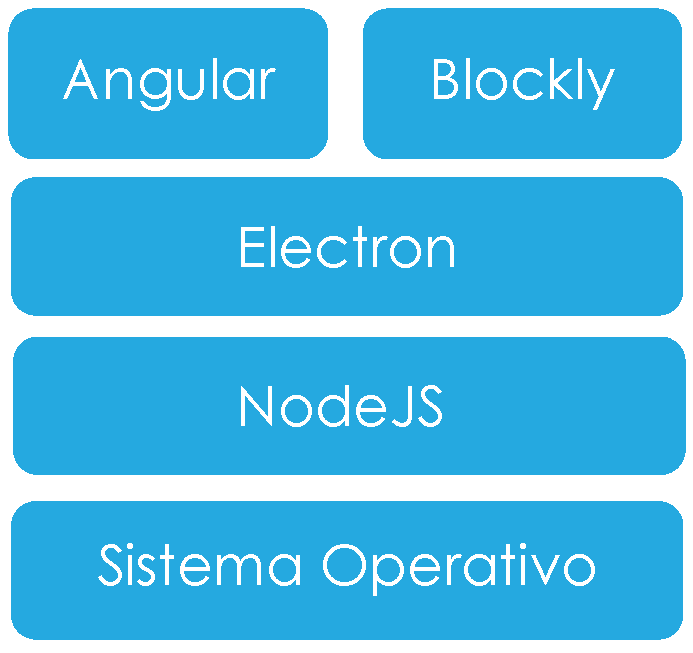
\includegraphics[scale=.8]{./Figures/ide-layers.pdf}
    \label{fig:ideLayers}
    \captionof{figure}{Distribución en capas de las tecnologías utilizadas.}
\end{center}

NodeJS es un entorno de ejecución de JavaScript que utiliza el motor V8 de Google. Utiliza un modelo de entradas y salidas no bloqueante y orientado a eventos. Esto y la posibilidad de utilizar múltiples hilos de ejecución, lo hacen ideal para el desarrollo de aplicaciones que requieran escalar.

Sobre las tecnologías arriba descritas se utilizó \emph{Angular}\citep{angular}, una plataforma para desarrollar aplicaciones web en HTML y JavaScript, o algún lenguaje que compile en JavaScript como TypeScript. La biblioteca consiste en varias bibliotecas modularizadas. 

La arquitectura de Angular consiste en \emph{plantillas} (\emph{templates}) HTML con una sintaxis especial, clases de \emph{componentes} que manejan estas plantillas y lo que muestran, \emph{servicios} que manejan la lógica de la aplicación y \emph{módulos} que engloban estos dos últimos. En general las aplicaciones tienen varios módulos que se incluyen en un módulo principal que inicia la aplicación.

Los componentes manejan en general pequeñas porciones de \emph{vistas} dentro de la aplicación (como ser navegaciones, listas dinámicas entre otras). Las plantillas, utilizando directivas, permiten mostrar propiedades del componente y actualizarlo a medida que éstas lo hagan. A su vez, informa al componente de los eventos ocurridos para que pueda reaccionar ante ellos. Esta dinámica se esquematiza en la figura \ref{fig:angularComponent}.

\begin{center}
    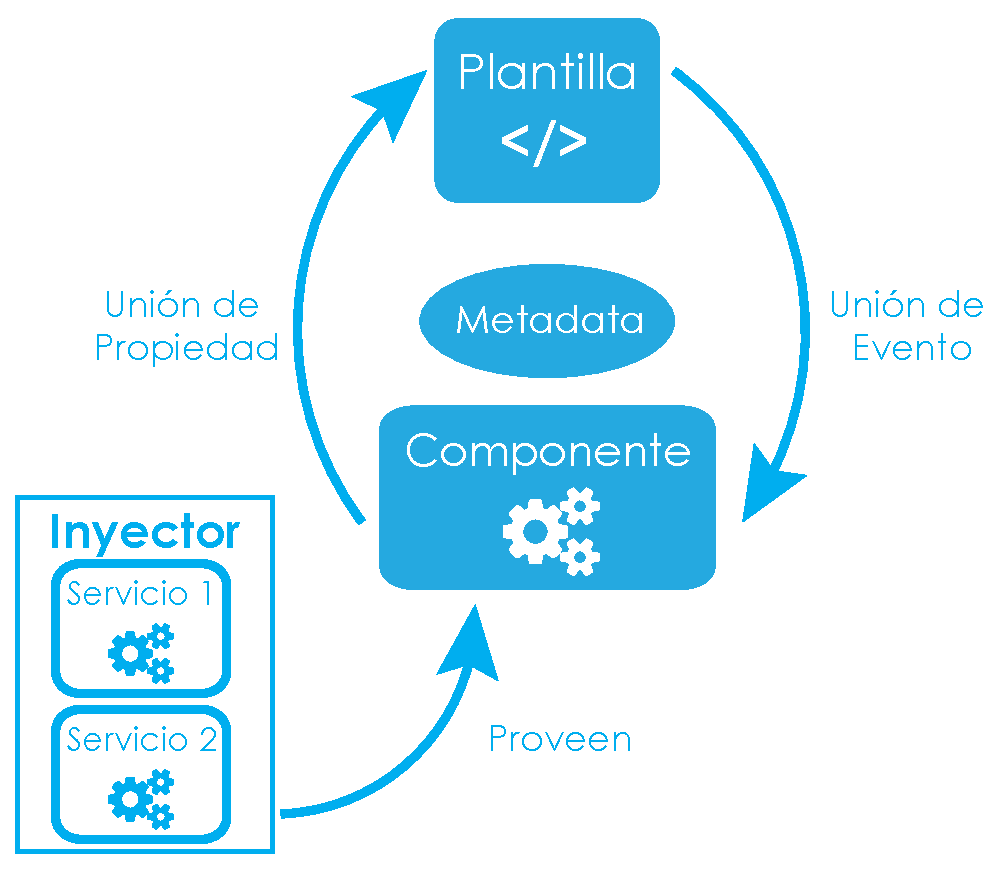
\includegraphics[scale=.7]{./Figures/componente-angular.pdf}
    \captionof{figure}{Interacción entre componente, plantilla y servicios en Angular.}
    \label{fig:angularComponent}
\end{center}

Los servicios intentan crearse con funciones puntuales y bien definidas. Los servicios son generalmente consumidos por componentes o incluso por otros servicios. Ejemplos de posibles usos son: 
\begin{itemize}
\item Manejo de datos.
\item Bus de mensajes.
\item Configuración de la aplicación.
\item Acceso a repositorio de datos.
\end{itemize}

Angular utiliza inyección de dependencias para proveer a las clases de las instancias de clases de las que depende. En general estas clases son servicios, se crea una instancia de ellos y se utiliza en los componentes en los que se requiera.

Este modo de estructurar el código sigue el lineamiento de división de responsabilidades, donde se arman pequeñas clases (componentes y servicios) que cumplen una tarea determinada, puntual y bien acotada.

Siguiendo con la idea de separación de tareas, se crearon (entre otros) dos servicios: \emph{ProjectService} encargado de tareas inherentes al manejo del proyecto abierto, y \emph{CompilingService} que permite compilar el código C y programarlo en la placa. Estos archivos pueden encontrarse en la ruta \texttt{/src/app/providers} dentro del código fuente del proyecto, ya que proveen a componentes de servicios o funcionalidades.

ProjectService posee el método \texttt{createProject} que crea la estructura básica de carpetas descrita en la subsección \ref{subsec:estructura-proyecto}. Para esto recibe el directorio que el usuario seleccionó para guardar su proyecto y utiliza la API fs (\emph{file system}) de NodeJS para crear los archivos y carpetas requeridos. Además, agrega este proyecto nuevo a la lista de proyectos recientes, que se guarda con la configuración persistente del usuario.

Otro método importante que posee este servicio es \texttt{openService}, que recibe la ruta de un proyecto existente y lo abre. De él toma los datos básicos y la estructura de bloques guardada en XML. Si el usuario aplica cambios sobre el proyecto abierto y están sin guardar, este servicio se encarga de registrar esa situación, por ejemplo para emitir una alerta al momento de intentar cerrar la aplicación sin haber guardado previamente.

Finalmente, este servicio también se encarga del guardado de los proyectos en archivos con extensión .cbp.

\subsection{Compilación}
Como se mencionó en la subsección \ref{subsec:estructura-proyecto}, el proyecto base utiliza Firmware V2 que es un proyecto en base a makefile. Esto significa que se utiliza la herramienta \emph{make} para realizar las diferentes tareas. Make sirve para la gestión de dependencias, como las que existen entre los archivos que componen el código fuente de un programa, para manejar su generación automática.

La función básica de make es determinar qué partes de un programa requieren ser recompiladas, y se encarga de ejecutar los comandos necesarios para lograrlo. Los makefiles son los archivos que utiliza esta herramienta para saber cómo compilar los programas y de qué depende cada uno. Podría hacerse una analogía con una receta, donde se encuentran los pasos para obtener lo requerido.

Los makefiles tienen una forma de reglas, donde se especifica lo que se debe hacer para obtener un módulo. Por ejemplo, a continuación se muestra cómo se define un módulo \emph{juego}, que requiere que se creen tres archivos de tipo objeto (.o), y luego especifica los comandos que deben ejecutarse para poder obtenerlos:

\begin{lstlisting}[caption=Ejemplo de un objetivo en makefile]
juego : ventana.o motor.o bd.o
    gcc -O2 -c juego.c -o juego.o
    gcc -O2 juego.o ventana.o motor.o bd.o -o juego
\end{lstlisting}

Luego, si se ejecutara \texttt{make juego}, se evaluarían los archivos con cambios desde la última compilación, y si hubiese cambios se recompilarían. De manera similar, el makefile de Firmware V2 tiene objetivos para programar el archivo binario compilado directamente a la placa, invocando a la herramienta de debug OpenOCD.

Contando con este simple manejo que provee un proyecto basado en makefile, se armó el servicio compilingService. Posee tres métodos que valen la pena destacar por su importancia para la aplicación.

El método \texttt{createMainFile} es el encargado de reescribir el archivo \texttt{main.c} con los últimos cambios que el usuario introdujo en el diagrama de bloques en el editor. Básicamente toma el archivo y solicita a blockly el código generado por el diagrama actual, luego lo reescribe y guarda el archivo.

Luego, el \texttt{compileProgram} actualiza el archivo \texttt{main.c} llamando al método recién descrito, y ejecuta un proceso hijo. Este proceso hijo corre en paralelo al hilo principal de la aplicación y actúa de manera no bloqueante. Esta es una gran ventaja que proporciona trabajar con NodeJS, ya que muchas operaciones que interactúan con el sistema operativo son bloqueantes y si no se pudiese lanzar un hilo en paralelo la aplicación no respondería hasta que finalizaran. Este proceso hijo que se lanza ejecuta la herramienta make, invocando al objetivo de compilación presente en el Makefile.

Algo importante de destacar es que la variable de ambiente \emph{Path}, es decir las rutas donde se buscarán los ejecutables, es modificada para los procesos hijos de este servicio. En las opciones de la aplicación, el usuario puede seleccionar rutas adicionales de búsqueda para indicar dónde se deberían buscar las herramientas necesarias (compilador y debugger), como se puede apreciar en la figura \ref{fig:idePath}.

El proceso hijo recibe una función de \emph{callback}, que será llamada una vez finalizado. Recibirá como argumentos el posible error si existiese, y la salida estándar del proceso. En función del resultado se notifica al usuario con el servicio de notificaciones.

Por último, el método \texttt{downloadProgram} actúa de manera similar a \texttt{compileProgram}, solo que esta vez se invoca el objetivo de grabado en flash del binario ya compilado.

\begin{figure}[H]
\centering
\includegraphics[scale=.8]{./Figures/path.jpg}
\caption{Ejemplo de rutas de búsqueda adicionales en el IDE.}
\label{fig:idePath}
\end{figure}


\section{Diseño del poncho CIAABOT G1}
Como se mencionó en la sección \ref{sec:alcance}, formó parte del alcance el diseño de un poncho para adaptar a una maqueta o robot existente a la plataforma. Para esto se diseñó un poncho, una placa que se puede conectar a la EDU-CIAA-NXP para ampliar las funcionalidades.

En este caso, el primer modelo se llamó \emph{G1}. Se pensó en un robot que tuviera sensores infrarrojos, o algún otro que deba ser medido de manera proporcional por un ADC o que pudiese conectarse directamente a una entrada digital. Además, se colocaron tres conectores que corresponden a las salidas de servomotores (SERVO0 a SERVO2) de la placa. Esto puede servir para movimiento de actuadores o para apuntar sensores. La sección de conectores puede apreciarse en el recorte del esquemático de la figura \ref{fig:g1Conectores}.

\begin{figure}[H]
\centering
\includegraphics[scale=.4]{./Figures/g1-conectores.JPG}
\caption{Recorte del esquemático que muestra los conectores disponibles.}
\label{fig:g1Conectores}
\end{figure}


Para el movimiento se optó por colocar dos drivers A4988 de motores paso a paso, como los de la figura \ref{fig:a4988}. Cada uno permite manejar un motor, con tensiones de hasta 35V y corrientes de hasta 2A. Además, permiten realizar micro-pasos sobre el motor, con una resolución de hasta un dieciseisavo de paso.

\begin{figure}[H]
\centering
\includegraphics[scale=.4]{./Figures/a4988.jpeg}
\caption{Driver A4988 de motor paso a paso.}
\label{fig:a4988}
\end{figure}

Para la alimentación del robot se consideró el uso de baterías. Se diseño un circuito conmutador con el integrado LM2577adj (figura \ref{fig:g1Fuente}), para elevar la tensión a los 12V utilizados sobre los motores paso a paso. Además, se agregó un regulador lineal LM7805 para la alimentación de la placa EDU-CIAA-NXP, que a su vez cuenta con un regulador para obtener los 3,3V necesarios para la lógica.

\begin{figure}[H]
\centering
\includegraphics[scale=.6]{./Figures/g1-fuente.JPG}
\caption{Recorte del esquemático que muestra la fuente de alimentación.}
\label{fig:g1Fuente}
\end{figure}

En la figura \ref{fig:g1PCB} se puede observar el diseño preliminar del circuito impreso del poncho, realizado en dos capas.

\begin{figure}[H]
\centering
\includegraphics[scale=.8]{./Figures/g1-pcb.JPG}
\caption{Diseño del circuito impreso del poncho G1.}
\label{fig:g1PCB}
\end{figure}

\section{Herramientas}
\subsection{Git}
Al momento de realizar la planificación del presente trabajo, se evaluaron posibles riesgos, cuál sería su impacto y cómo deberían poder mitigarse, ya sea reduciendo su probabilidad de ocurrencia o su severidad.

Dentro de los riesgos planteados se consideró la pérdida de archivos importantes para el desarrollo de la aplicación. Se evaluó que su consecuencia sería muy severa ya que implicaría una pérdida muy grande de tiempo, que no podría recuperarse en el cronograma de trabajo. La estrategia de mitigación para este riesgo fue el uso constante y riguroso del sistema de control de versiones \emph{Git}.

Un sistema de control de versiones registra los cambios a uno o más archivos a lo largo del tiempo, para luego poder recuperar versiones específicas. Hay diferentes sistemas, hoy en día el más utilizado es Git.

Git es un sistema del tipo distribuido, esto quiere decir que los usuario toman la historia completa del repositorio cada vez que lo clonan del servidor, como se observa en la figura \ref{fig:repositorioDistribuido}. De esta manera cada computadora es una copia de seguridad completa del proyecto, y en caso de que el servidor sufriera problemas, las pérdidas serán casi nulas.

\begin{center}
    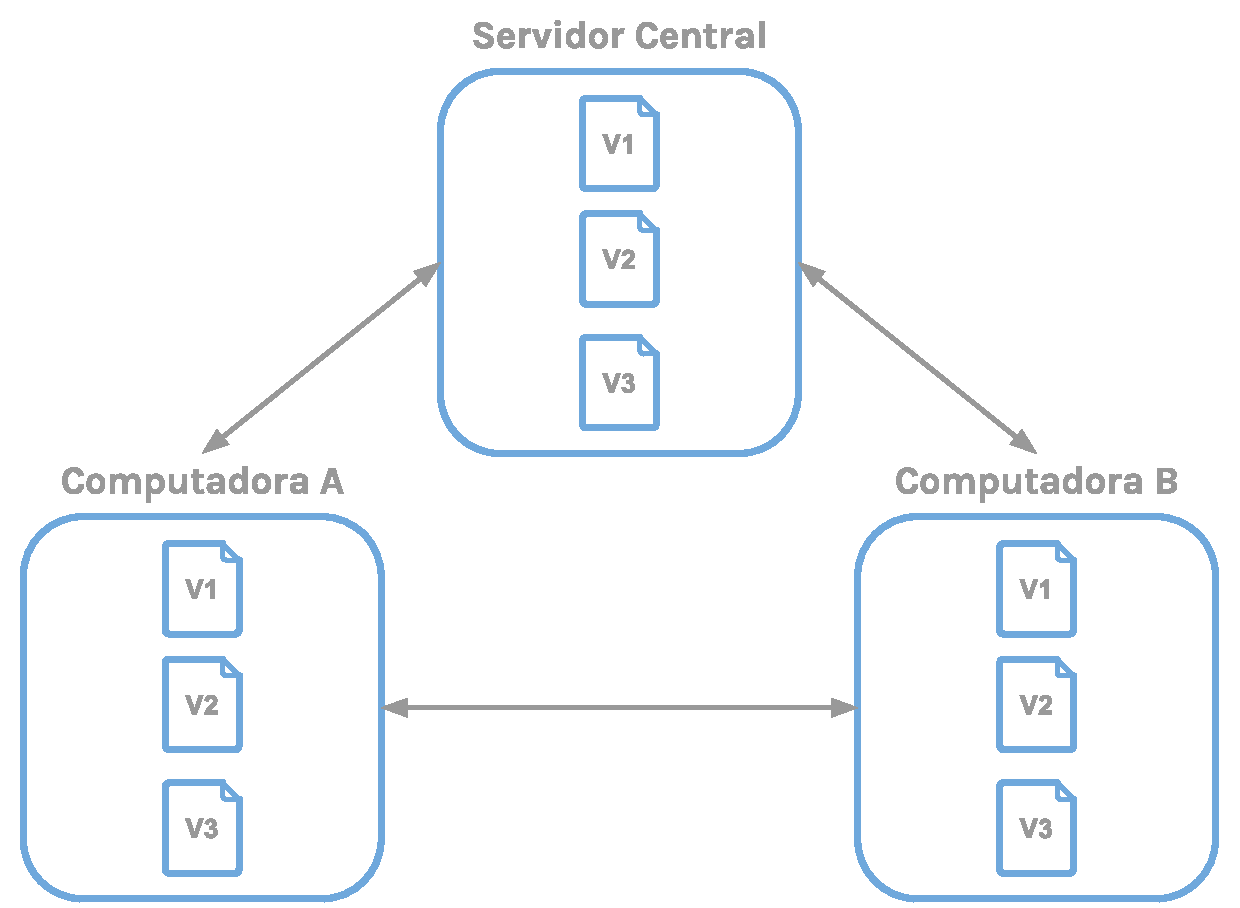
\includegraphics[scale=.6]{./Figures/repositorio-distribuido.pdf}
    \captionof{figure}{Diagrama de un repositorio distribuido. Cada computadora posee todas las versiones.}
    \label{fig:repositorioDistribuido}
\end{center}

El proyecto CIAABOT es abierto, y el código fuente para compilar o modificar el IDE se encuentra en GitHub \citep{CIAABOT:repositorio}. El desarrollo se separó en ramas en el repositorio, para un trabajo más puntual sobre diferentes características (pantalla de carga, rutas adicionales de búsqueda, variables tipadas, etc), y el código que debe considerarse estable se mantiene en la rama Master.

\subsection{OpenOCD}
Para el grabado del firmware en las placas y su posterior depuración, se utilizó la herramienta OpenOCD. Es un depurador libre \emph{on-chip}, creado por Dominic Rath. Utilizando entornos de desarrollo como Eclipse o Visual Studio Code, es posible depurar diferentes placas conectadas por puerto serie a la PC.

OpenOCD permite utilizar archivos de configuración para seleccionar la placa que se desea utilizar, lo cual es muy útil para CIAABOT ya que se espera que se puedan ampliar las placas soportadas del ecosistema CIAA.